\documentclass[10pt,a4paper]{article}
\usepackage[margin=22mm,headheight=27pt]{geometry}
\usepackage[T1]{fontenc}
\usepackage{lmodern,microtype}
\usepackage{graphicx,booktabs,longtable,tabularx,array}
\usepackage{amsmath}
\usepackage{tikz}
\usetikzlibrary{arrows.meta,positioning,fit,backgrounds,calc}
\usepackage{pdflscape}
\usepackage{listings,needspace}
\usepackage{xcolor,fancyhdr}
\usepackage{caption}
\usepackage[hidelinks]{hyperref}
\usepackage{xurl}
\definecolor{aegis}{HTML}{0B5D4B}
\definecolor{rulegray}{gray}{0.75}
\definecolor{codegray}{gray}{0.96}
\hypersetup{pdftitle={AEGIS: API Workflow and Data Delivery},pdfauthor={Ilias Akritidis, Georgios Mallousis, Vasileios Sevetlidis}}
\pagestyle{fancy}
\fancyhf{}
\fancyhead[L]{\small AEGIS: API Workflow}
\fancyhead[R]{\footnotesize\begin{tabular}{@{}r@{}}ARGUS Open Innovation Challenge 2026\\Track A: Heritage and Citizen Science\end{tabular}}
\fancyfoot[C]{\small\thepage}
\renewcommand{\headrulewidth}{0.3pt}
\setlength{\parskip}{0.35em}
\setlength{\parindent}{1em}
\setlength{\emergencystretch}{2em}
\setlength{\textfloatsep}{13pt}
\captionsetup{font=small,labelfont=bf}
\newcolumntype{Y}{>{\raggedright\arraybackslash}X}
\lstset{basicstyle=\ttfamily\footnotesize,backgroundcolor=\color{codegray},frame=single,rulecolor=\color{rulegray},breaklines=true,columns=fullflexible,keepspaces=true,showstringspaces=false,aboveskip=0.6em,belowskip=0.6em}
\tikzset{box/.style={draw=black!65,rounded corners=1pt,fill=white,align=center,font=\small,inner sep=5pt},flow/.style={-{Latex[length=2mm]},draw=black!75},optional/.style={flow,dashed},tag/.style={font=\scriptsize,align=center,fill=white,inner sep=2pt}}

\begin{document}
\fontsize{10.5}{13}\selectfont
\begin{center}
{\LARGE\bfseries AEGIS: API Workflow and Data Delivery\par}
\vspace{0.5em}
{\large Technical Deliverable\par}
\vspace{0.6em}
Ilias Akritidis\textsuperscript{*}, Georgios Mallousis\textsuperscript{*}, Vasileios Sevetlidis\par
\vspace{0.3em}
{\small International Hellenic University, Polytechnic School\\
Department of Computer, Informatics and Telecommunications Engineering\par}
{\small\href{mailto:iliakrit@ihu.gr}{\texttt{iliakrit@ihu.gr}}\quad
\href{mailto:geomallo@ihu.gr}{\texttt{geomallo@ihu.gr}}\quad
\href{mailto:vasiseve@ihu.gr}{\texttt{vasiseve@ihu.gr}}\par}
\vspace{0.6em}
\end{center}
{\renewcommand{\thefootnote}{\fnsymbol{footnote}}\footnotetext[1]{Ilias Akritidis and Georgios Mallousis contributed equally to this work.}}


\section{Purpose and scope}
AEGIS uses ARGUS monitoring data to connect decisions made during gameplay with the preservation needs of five heritage sites. The API workflow supplies the site's risk scenarios, the instruments installed there, and recorded alarms that the game can explain. It also provides recent monitoring information for the opening screen. AEGIS implements these functions through a stable gameplay dataset and a separate mechanism for incorporating new records.

The scope encompasses snapshot acquisition, incremental collection, data preparation, publication and browser consumption.\footnote{Implementation baseline: source revision \texttt{b61c190} on branch \texttt{readyToSubmit}. Entry points: \path{tools/fetch_snapshot.py}, \path{tools/build_game_data.py}, \path{tools/pi/guardian_live.py}, \path{.github/workflows/site.yml}, and \path{web/src/game/live.ts}. File paths in implementation footnotes are relative to the AEGIS repository.} Verification addresses the processing logic and retained data; the operational availability of the ARGUS API and external delivery services lies outside the reported assessment. The associated data-analysis documentation describes the interpretation and selection of monitoring records.\footnote{Data-analysis methodology: \path{doc/data-analysis/README.md}.}

\section{Literature and design rationale}
Reproducible computational work requires more than a description of an algorithm. Sandve et al. recommend retaining the information needed to reconstruct each result, including the versions of data, software and analysis procedures~\cite{sandve2013}. Wilson et al. similarly emphasise version control, automated workflows, testing and documentation of interfaces and design decisions~\cite{wilson2014}. These recommendations motivate the retention of AEGIS inputs and executable preparation steps. The W3C PROV model distinguishes data entities, processing activities and responsible agents, providing a basis for explaining how an output was derived~\cite{prov2013}.

The Dataflow model distinguishes the time of an event from the time at which a processing stage observes it, and examines the trade-offs between correctness, latency and processing cost~\cite{akidau2015}. This distinction is relevant to AEGIS even though its collector is currently a periodic script. An assessment can be collected and published long after it was produced. Source timestamps, collection time and publication time are therefore distinguished throughout the workflow. Freshness limits and collection intervals form part of its operational configuration.

Reliability guidance also cautions that retries can amplify load when an upstream service is already failing. Ulrich recommends bounded retries, backoff and deliberate degradation of optional functionality~\cite{ulrich2016}. AEGIS applies request limits and retains the core game when recent monitoring data is unavailable. This separation applies the principle of retaining essential functionality during a dependency failure. The suitability of individual request limits remains subject to operational evaluation.

\section{System architecture}
The integration comprises a snapshot acquisition path and an incremental monitoring path. Snapshot acquisition supplies the records required for mission construction, alarm interpretation and representation of the installed sensor networks. The incremental service, hosted on a Raspberry Pi, retrieves recent risk evaluations and alarms. During publication, GitHub Actions combines the application build with a copy of the recent monitoring data to produce a static deployment. The browser accesses these published resources through the application endpoint, \textbf{with no direct dependency on the ARGUS API during gameplay}. Figure~\ref{fig:context} presents the system context, and Figure~\ref{fig:containers} identifies the components responsible for acquisition, processing and delivery.

\begin{figure}[htbp]
\centering
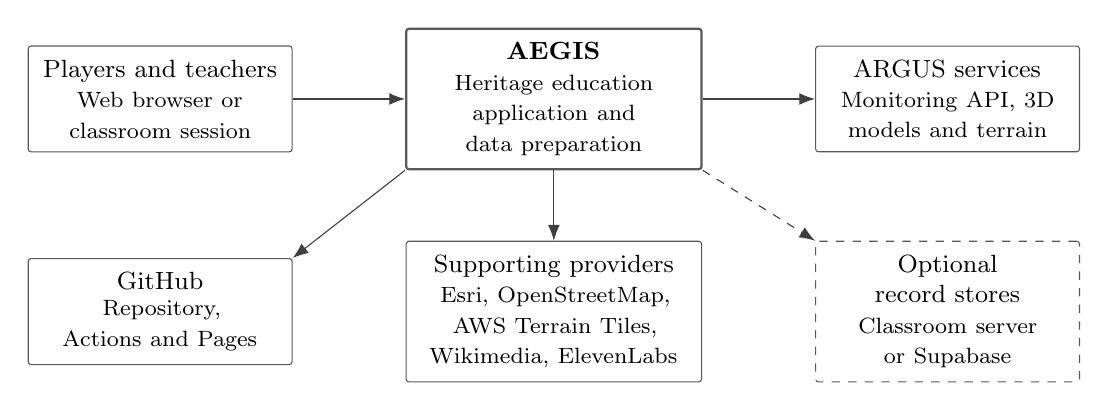
\begin{tikzpicture}[x=1cm,y=1cm]
\node[box,text width=3.0cm] (users) at (-5,2.0) {Players and teachers\\\footnotesize Web browser or classroom session};
\node[box,text width=3.4cm,line width=.8pt] (aegis) at (0,2.0) {\textbf{AEGIS}\\\footnotesize Heritage education application and data preparation};
\node[box,text width=3.0cm] (argus) at (5,2.0) {ARGUS services\\\footnotesize Monitoring API, 3D models and terrain};
\node[box,text width=3.0cm] (github) at (-5,-0.7) {GitHub\\\footnotesize Repository,\\Actions and Pages};
\node[box,text width=3.4cm] (assets) at (0,-0.7) {Supporting providers\\\footnotesize Esri, OpenStreetMap, AWS Terrain Tiles, Wikimedia, ElevenLabs};
\node[box,text width=3.0cm,dashed] (optional) at (5,-0.7) {Optional record stores\\\footnotesize Classroom server or Supabase};
\draw[flow] (users) -- (aegis);
\draw[flow] (aegis) -- (argus);
\draw[flow] (aegis.south west) -- (github.north east);
\draw[flow] (aegis) -- (assets);
\draw[optional] (aegis.south east) -- (optional.north west);
\end{tikzpicture}

\caption{System context. ARGUS supplies monitoring records and spatial assets. AEGIS prepares and publishes these resources for players and teachers. Dashed connections denote optional classroom or shared-storage services.}
\label{fig:context}
\end{figure}

The browser application uses React, TypeScript, Leaflet, and three.js. A service worker supports the offline core game. A dedicated preparation environment performs snapshot acquisition, retrieves the required spatial assets and generates the application data packs. The Raspberry Pi executes a scheduled Python reader and exposes its output through Caddy and a playit.gg tunnel. GitHub provides source storage, automated checks, and static delivery. Caddy can also serve the built game; its live-data route reads from a separate directory so that publishing a new site does not replace the collector's state\footnote{Deployment configuration: \path{tools/pi/guardian-live.service}, \path{tools/pi/guardian-live.timer}, \path{tools/pi/Caddyfile}, and \path{tools/pi/README.md}.}.

\section{Interfaces and acquisition}
\subsection{ARGUS records}
The acquisition scripts target \url{http://api.argusservices.athenarc.gr/api}. They use paginated JSON responses containing \texttt{data} and \texttt{meta}, including \texttt{last\_page} and \texttt{total}. The implementation assumes pages contain 15 records in ascending order. Table~\ref{tab:endpoints} lists the resources used by AEGIS. All of these acquisition requests use \texttt{GET}. RFC~9110 defines \texttt{GET} and \texttt{HEAD} as safe and idempotent methods, supporting retrieval and the repetition of requests after communication failures~\cite{http2022}. Idempotence concerns the intended server-side effect; it does not guarantee identical responses from a changing dataset.

The snapshot fetcher sends an identifying \texttt{User-Agent} and requests JSON. When \path{ARGUS_API_TOKEN} is present in the environment, it also sends an \texttt{Authorization: Bearer} header. The live reader sends an identifying \texttt{User-Agent} and accepts JSON, but currently implements no authentication-header mechanism. Authentication requirements are governed by the access policy of the ARGUS deployment; the request mechanisms described here reflect the acquisition clients' configuration.

{\small
\begin{longtable}{@{}p{0.29\textwidth}p{0.16\textwidth}p{0.48\textwidth}@{}}
\caption{ARGUS resource catalogue. Paths are relative to \texttt{/api}; paginated calls append \texttt{?page=N}. S: snapshot acquisition; L: incremental reader; R: retained reference snapshot.}\label{tab:endpoints}\\
\toprule
Resource & Consumer & Role in AEGIS\\
\midrule\endfirsthead
\toprule Resource & Consumer & Role in AEGIS\\\midrule\endhead
\bottomrule\endfoot
\path{/assets} & S & Identifies the five heritage sites.\\
\path{/asset-states} & S & Site metadata and placements of spatial representations.\\
\path{/threats} & S & Risk scenarios, categories, ABC scores and priorities.\\
\path{/threat-contexts} & S, L & Risk evaluations, probabilities, states and thresholds.\\
\path{/events} & S, L & Expert-rule and AI alarms, timestamps, readings and explanatory feature contributions.\\
\path{/policies} & S & Alarm rules and current policy thresholds.\\
\path{/installed-instruments} & S & Instrument identifiers, names and location descriptions.\\
\path{/installed-devices} & S & Installed-device coordinates.\\
\path{/instruments} & S & Links instruments to their types.\\
\path{/instrument-types} & S & Instrument-type names used in sensor-card mappings.\\
\path{/decisions} & S; R fallback & Decisions recorded after alarms.\\
\path{/decision-contexts} & S; R fallback & Relationships between decisions and alarms.\\
\path{/monitorings} & R & Sensor placements in the ARGUS three-dimensional viewer.\\
\end{longtable}}

\subsection{Spatial and supporting resources}
The spatial fetcher reads the ARGUS terrain descriptors and tiles under \path{/terrain/<monument>/} and the 3D Tiles descriptors and models under \path{/tiles/<model>/}. It uses \texttt{HEAD} requests to estimate model-tile sizes before downloading them with \texttt{GET}. The default model budget is 8\,MB per scene. Terrain extraction uses a default 2\,m grid, with a maximum acquisition radius of 300\,m in the all-scenes mode. These settings bound the spatial subset packaged with the application; they do not describe the full resolution or extent of the upstream datasets. The client checks \texttt{robots.txt} before accessing the configured host\footnote{Spatial acquisition and scene preparation: \path{tools/fetch_argus_3d.py}, \path{tools/build_preview_3d.py}, and \path{tools/build_scenes_3d.py}.}.

Additional services support presentation. Esri World Imagery and OpenStreetMap supply map backgrounds, while AWS Terrain Tiles and Wikimedia Commons support parts of the 3D experience. The OpenStreetMap API supplies outlines used in packaged fallback plans. An offline recording process can generate narration through ElevenLabs; playback uses the resulting audio files. Optional Supabase storage and the local classroom server concern player records, not writes to ARGUS. They remain distinct from the monitoring acquisition path.

\begin{figure}[p]
\centering
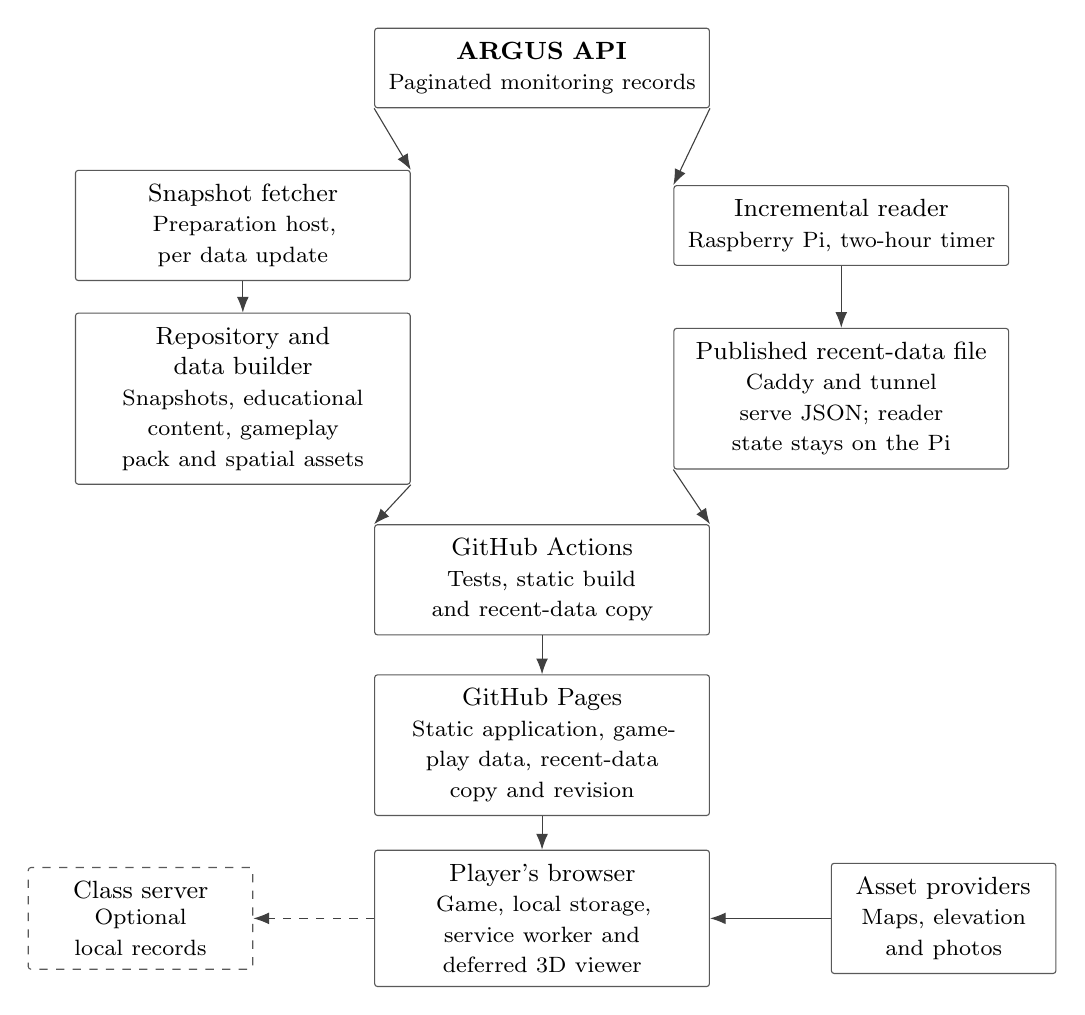
\begin{tikzpicture}[x=1cm,y=1cm]
\node[box,text width=3.9cm] (api) at (0,0) {\textbf{ARGUS API}\\\footnotesize Paginated monitoring records};
\node[box,text width=3.9cm] (snapshot) at (-3.8,-2.0) {Snapshot fetcher\\\footnotesize Preparation host, per data update};
\node[box,text width=3.9cm] (reader) at (3.8,-2.0) {Incremental reader\\\footnotesize Raspberry Pi, two-hour timer};
\node[box,text width=3.9cm] (repo) at (-3.8,-4.2) {Repository and data builder\\\footnotesize Snapshots, educational content, gameplay pack and spatial assets};
\node[box,text width=3.9cm] (public) at (3.8,-4.2) {Published recent-data file\\\footnotesize Caddy and tunnel serve JSON; reader state stays on the Pi};
\node[box,text width=3.9cm] (actions) at (0,-6.5) {GitHub Actions\\\footnotesize Tests, static build and recent-data copy};
\node[box,text width=3.9cm] (pages) at (0,-8.6) {GitHub Pages\\\footnotesize Static application, gameplay data, recent-data copy and revision};
\node[box,text width=3.9cm] (browser) at (0,-10.8) {Player's browser\\\footnotesize Game, local storage, service worker and deferred 3D viewer};
\node[box,text width=2.5cm,dashed] (class) at (-5.1,-10.8) {Class server\\\footnotesize Optional\\local records};
\node[box,text width=2.5cm] (tiles) at (5.1,-10.8) {Asset providers\\\footnotesize Maps, elevation and photos};
\draw[flow] (api.south west) -- (snapshot.north east);
\draw[flow] (api.south east) -- (reader.north west);
\draw[flow] (snapshot) -- (repo);
\draw[flow] (reader) -- (public);
\draw[flow] (repo.south east) -- (actions.north west);
\draw[flow] (public.south west) -- (actions.north east);
\draw[flow] (actions) -- (pages);
\draw[flow] (pages) -- (browser);
\draw[optional] (browser) -- (class);
\draw[flow] (tiles) -- (browser);
\end{tikzpicture}

\caption{Component and data-delivery view. The snapshot and incremental paths converge during publication. State used by the live reader remains on the Pi, while only its public JSON output enters the website. Optional classroom storage does not communicate with the ARGUS API.}
\label{fig:containers}
\end{figure}

\section{Processing and data contracts}
\subsection{Snapshot preparation}
\path{tools/fetch_snapshot.py} retrieves twelve resources, following each response's \texttt{meta.last\_page}. It pauses 0.25\,s between page requests by default and allows four attempts per request, with waits of 2, 4 and 6\,s after failures. Each request has a 90\,s timeout. Records are deduplicated by identifier and sorted before writing. The output records the resource name, count, completeness flag, collection time, and records. Completeness means that the unique count reaches or exceeds the final reported total. This way the complete count avoids being an atomic transaction across the API. The script refuses to overwrite the original reference snapshot or an existing non-empty destination.

\path{tools/build_game_data.py} selects the newest available snapshot using its recorded collection metadata and combines it with the educational content used in the application. The retained snapshot dated 12 October 2026 supplies the ten core resource types. Decisions and decision contexts fall back to the original snapshot when absent from the selected input. The spatial scene builder also uses retained monitoring records for viewer placements. Fields drawn from a reference snapshot need not share the collection date shown for the core dataset. Recording that distinction preserves the derivation history needed to interpret a combined output, consistent with the provenance concepts described by PROV-DM~\cite{prov2013}.

The builder produces \path{web/public/data/game_data.json} and \path{docs/data_notes.md}. The former contains the subset needed by the game, including site information, mission risks, sensor mappings, interpretable alarms and their validation rules. The latter records data counts, exclusions and assumptions. Raw asset-state records remain preparation inputs and are not requested by the browser. The detailed rules for alarm filtering and mission construction belong to the accompanying data-analysis deliverable\footnote{Data preparation and analysis documentation: \path{tools/build_game_data.py}, \path{docs/data_notes.md}, and \path{doc/data-analysis/README.md}.}.

\subsection{Incremental collection}
The live service reads only \path{threat-contexts} and \path{events}. For each resource, its cursor stores the last page examined, greatest record identifier, and reported total. A later run revisits the saved page to detect records added to a previously incomplete page, then continues forward. It accepts records with identifiers greater than the saved identifier and processes at most 400 pages per resource per run. Requests are 0.5\,s apart; each allows three attempts with waits of 5 and 10\,s and a 30\,s timeout\footnote{Incremental-reader parameters and cursor logic: \path{tools/pi/guardian_live.py}.}.

If the reported total or page count falls below the saved position, the reader clears the affected resource's state and reads it again from the beginning. This mechanism detects shrinking collections. It does not identify every possible upstream edit, particularly an in-place revision with an unchanged identifier and total.

The reader retains the latest evaluation for each scenario and the ten newest distinct alarms per site. Alarm identity combines its type, rule, timestamp and signal names. When constructing the published risk view, it groups evaluations within twelve hours of the newest evaluation at each site. This heuristic limits the published risk view to evaluations near the newest retained assessment. The configured window establishes temporal proximity between evaluations; membership of a common upstream assessment run remains unverified.

The service writes \texttt{state.json} for its next run and \texttt{public/argus-now.json} for publication. Each file is written through a temporary file followed by an atomic replacement. If collection fails, the program returns without replacing the previous published file. Atomic replacement applies to each file independently; the state and public output are committed in separate operations.

\subsection{Published recent-data contract}
The top-level JSON object contains \texttt{schema}, \texttt{source}, \texttt{checked\_at}, and \texttt{sites}. Schema version 1 identifies the current contract. Each site may contain a risk object and an alarm list. The risk object carries the latest evaluation time and its scenario evaluations. Alarm entries retain their timestamp, type, applicable rule, variables, model score and threshold, and leading feature contribution when available. Fields are reduced to those needed by the browser, and individual copied strings are bounded in length.

Risk timestamps with timezone information are normalised to UTC. Alarm timestamps are retained in ARGUS's timezone-free form; the browser interprets those values as UTC. RFC~3339 identifies unqualified local times as an interoperability problem and specifies timestamps with an explicit relationship to UTC~\cite{timestamps2002}. The interpretation of timezone-free alarm values as UTC is an integration assumption requiring confirmation against the provider's timestamp convention. The file's \texttt{checked\_at} value describes collection, whereas the nested evaluation and alarm times describe the source events. A recent collection time therefore does not imply that a new assessment occurred at every site. This is an instance of the event-time and processing-time distinction described by Akidau et al.~\cite{akidau2015}.

\section{Publication and browser consumption}
\subsection{Build and static delivery}
The publication workflow runs on pushes to \texttt{main}, by manual dispatch, and on a nightly schedule at 23:00 UTC. It executes the Python data tests, installs the locked web dependencies, runs the web tests, and builds the application with TypeScript and Vite. A failure prevents the subsequent publication steps\footnote{Build, validation, fallback and publication steps: \path{.github/workflows/site.yml}.}.

After the build, GitHub Actions requests the Pi's published JSON through an address supplied by the repository secret \texttt{PI\_LIVE\_URL}. It accepts a file only if it is valid JSON with \texttt{schema=1} and an object-valued \texttt{sites} field. This is a structural gate, not full semantic validation of every nested record. If the request or validation fails, the workflow attempts to retain the previous deployed copy. With no valid copy, it publishes the core application without recent monitoring information.

The workflow commits the static output to the \texttt{site} branch and writes the source revision to a \texttt{VERSION} file. GitHub Pages serves that branch over HTTPS. The Pi's two-hour timer and the website's publication schedule are separate, so browser requests obtain the file copied at the last successful build. Figure~\ref{fig:sequence} summarises the request sequence.

\subsection{Selection and freshness}
The browser reads \path{data/game_data.json} and requests \path{live/argus-now.json} with an 8\,s timeout. The live-file loader reuses its in-memory promise for ten minutes, limiting repeated fetches when it is called again. This cache interval is not a guarantee that the interface automatically polls every ten minutes. Nested parsing rejects or omits unusable records before they reach the display\footnote{Browser parsing and display: \path{web/src/game/live.ts} and \path{web/src/components/LiveArgus.tsx}.}.

Risk checks remain eligible for fourteen days. Checks no older than 36 hours can receive the ``Live from ARGUS'' label; older eligible checks receive a less immediate label. Alarm entries remain eligible for sixty days and must pass the same interpretability and plausibility rules supplied by the data builder. An AI alarm, for example, requires a sufficiently dominant feature that maps to a supported sensor explanation. The interface may show an eligible risk view or an interpretable alarm; if neither is available, the recent-data component is omitted while gameplay continues. Values more than one hour in the future are also excluded. The eligibility periods and clock tolerance are application-level display parameters, distinct from the thresholds used by the ARGUS risk models.

\subsection{Offline and deferred resources}
The service worker stores the core application's build assets and data. It retrieves the data pack from the network first and falls back to its cached copy when the request fails. The recent-data route is network-only and is excluded from service-worker caching. External map tiles are not cached by the application, and the map uses its packaged plans when imagery is unavailable\footnote{Service-worker caching and build exclusions: \path{web/sw-template.js} and \path{web/vite.config.ts}.}.

The three-dimensional viewer loads its scene descriptions, models and terrain on demand. Its code and scene data are excluded from the initial offline pack, and external imagery, elevation tiles or photographs may still require connectivity. Audio clips are cached individually after playback and they are not downloaded in full at installation. Consequently, offline support applies to the core game after a successful first visit, not to every optional resource.

\section{Reliability, security and operational limits}
Table~\ref{tab:limits} consolidates the implemented request limits. Bounded retries can recover from some transient failures, while fallback allows the core game to continue without recent monitoring data. The request backoff is linear, whereas the reliability guidance recommends randomised exponential backoff to reduce synchronised retry load~\cite{ulrich2016}. The timer's scheduling jitter does not provide request-level jitter. Request-level retry behaviour therefore remains a candidate for further refinement. Recovery of a large backlog may span several collection runs, depending on the volume accumulated during an interruption.

\begin{table}[htbp]
\centering\small
\caption{Configured acquisition and delivery limits. Parameters refer to the acquisition and delivery configuration; they do not constitute service-level guarantees.}\label{tab:limits}
\begin{tabularx}{\textwidth}{@{}p{0.23\textwidth}YYY@{}}
\toprule Component & Spacing or schedule & Timeout & Attempts or bound\\\midrule
Snapshot fetcher & 0.25\,s between pages & 90\,s per request & 4 attempts; waits 2, 4, 6\,s\\
Incremental reader & 0.5\,s between pages; 2\,h timer & 30\,s per request & 3 attempts; 400 pages per resource per run\\
Pi service & First run after boot, about 2\,min; up to 1\,min jitter & 15\,min per service invocation & Retains prior output after collection failure\\
Actions live copy & At each successful build & 30\,s download & Prior valid deployment copy as fallback\\
Browser live loader & 10\,min in-memory reuse interval & 8\,s & No service-worker caching of the live file\\
\bottomrule
\end{tabularx}
\end{table}

The acquisition configuration uses HTTP for ARGUS record requests and HTTPS for the public website. The Pi's transfer through the configured tunnel can also use HTTP. The transport protection of the public delivery endpoint consequently does not extend to every upstream transfer. The snapshot client reads an optional bearer token from the environment and does not write it into its snapshot files; its use must follow the access arrangements supplied by ARGUS. Supplying a credential through the environment avoids embedding it in source files but does not protect it during transmission. RFC~6750 requires TLS or equivalent transport security for bearer-token requests~\cite{bearer2012}. The optional bearer-token path should therefore use a protected transport.

The Pi reader runs as a dedicated system user with its own state directory. The systemd unit specifies a read-only system, protected home directories, private temporary storage and devices, restricted capabilities, and a fifteen-minute runtime limit. Restricting the reader to the permissions needed for its task follows the least-privilege principle articulated by Saltzer and Schroeder~\cite{saltzer1975}. The service configuration specifies the corresponding access restrictions; an independent security assessment remains outside the scope of the verification\footnote{Deployment configuration: \path{tools/pi/guardian-live.service}, \path{tools/pi/guardian-live.timer}, \path{tools/pi/Caddyfile}, and \path{tools/pi/README.md}.}.

All interactions with the ARGUS record API are read-only. Player choices, scores and observations do not enter that API. In the default device-storage mode, these records remain in browser storage. An explicitly configured classroom server or shared store introduces a separate destination for supported player records. Observation reports leave the device through an explicit user action, such as saving, printing or preparing an email. These optional record-sharing functions operate independently of the monitoring feed and preserve the separation between heritage-data acquisition and player-generated information.

\Needspace{18\baselineskip}
\section{Reproducibility and verification}
\subsection{Local reproduction}
The data tools require Python 3.9 or later and use the standard library. The web application requires Node.js 20 or later and installs its dependencies from \path{web/package-lock.json}. The committed snapshots and packaged data allow local inspection without contacting ARGUS. Retaining the original inputs, software revision and executable preparation commands supports the reconstruction of computational results advocated by Sandve et al.~\cite{sandve2013}. The following commands run from the repository root and validate the existing pack before building and serving the application:
\begin{lstlisting}
python3 -I tools/build_game_data.py --check
python3 -I -m unittest discover -s tools/tests -t tools
cd web
npm ci
npm test
npm run build
npm run preview
\end{lstlisting}

\noindent Omitting \texttt{--check} in the first command regenerates the pack from the selected retained snapshot. To acquire a fresh snapshot, run the following with the access configuration supplied by the organiser; the destination must be new or empty:
\begin{lstlisting}
python3 -I tools/fetch_snapshot.py --out snapshot_review
python3 -I tools/build_game_data.py --snapshot snapshot_review
python3 -I tools/build_preview_3d.py
python3 -I tools/build_scenes_3d.py
python3 -I tools/fetch_argus_3d.py all
\end{lstlisting}

\noindent The new snapshot command retrieves twelve resources; it does not recreate the original collection of all ARGUS resources. Spatial generation still requires the retained monitoring and placement inputs. Network-backed commands also depend on the continued availability and permitted use of upstream services. Fallback map plans and narration have their own preparation tools, \path{tools/fetch_backdrops.py} and \texttt{npm run narration}, respectively.

A single incremental collection can run on any suitable computer, independently of systemd:
\begin{lstlisting}
python3 -I tools/pi/guardian_live.py --out /tmp/aegis-live-review
\end{lstlisting}

\noindent This creates \path{/tmp/aegis-live-review/state.json} and \path{/tmp/aegis-live-review/public/argus-now.json}; it does not publish them automatically. Deployment of the Pi service uses the supplied systemd unit, timer and Caddy configuration. Publication to GitHub Pages uses the repository workflow and its configured live-file address. The optional classroom server can serve a built game locally with \texttt{python3 -I tools/class\_server.py}; LAN access requires its explicit \texttt{--lan} option.

% \subsection{Verification evidence}
% Verification conducted on 25 October 2026 comprised nine Python tests for the incremental reader, twelve browser-logic tests for recent monitoring data, and validation of the retained game-data pack. All checks completed successfully. The Python tests exercise incremental retrieval, reset behaviour, deduplication, invalid-record handling, site-specific evaluation windows, preservation of output after failure, and consistency with the snapshot. The browser tests cover parsing, freshness and alarm selection, including agreement with the builder's retained alarms\footnote{Test implementations: \path{tools/tests/test_guardian_live.py} and \path{web/tests/live.test.ts}. The retained pack was checked with \texttt{python3 -I tools/build\_game\_data.py --check}.}.

% Wilson et al. describe automated tests as checks of expected behaviour at unit, integration and regression levels~\cite{wilson2014}. The reported results provide evidence for the tested logic against retained inputs and simulated API responses. They do not measure API uptime, verify the running Pi, establish deployment freshness, or replace a complete browser and security assessment. The source files and generated outputs identify the implementation and data used, while the deployed \texttt{VERSION} file provides a means of checking which revision a public site actually serves.

\section{Conclusion}
The workflow supports a reproducible educational application by separating the preparation of gameplay data from the collection of recent monitoring records. A static publication step gives the browser a compact interface to ARGUS-derived information, while retained inputs and fallback behaviour preserve the core experience when upstream services are unavailable. Its principal operational constraints are the assumptions of the incremental reader, the delay introduced by publication, the HTTP acquisition paths, and the connectivity needed by optional spatial resources. These constraints define the conditions under which the delivered workflow should be reproduced and interpreted.

\begin{thebibliography}{9}
\small
\bibitem{sandve2013} G.~K. Sandve, A. Nekrutenko, J. Taylor, and E. Hovig, ``Ten Simple Rules for Reproducible Computational Research,'' \emph{PLOS Computational Biology}, vol.~9, no.~10, e1003285, 2013. \url{https://doi.org/10.1371/journal.pcbi.1003285}.
\bibitem{wilson2014} G. Wilson et al., ``Best Practices for Scientific Computing,'' \emph{PLOS Biology}, vol.~12, no.~1, e1001745, 2014. \url{https://doi.org/10.1371/journal.pbio.1001745}.
\bibitem{prov2013} L. Moreau and P. Missier, eds., \emph{PROV-DM: The PROV Data Model}. W3C Recommendation, 30 April 2013. \url{https://www.w3.org/TR/2013/REC-prov-dm-20130430/}.
\bibitem{akidau2015} T. Akidau et al., ``The Dataflow Model: A Practical Approach to Balancing Correctness, Latency, and Cost in Massive-Scale, Unbounded, Out-of-Order Data Processing,'' \emph{Proceedings of the VLDB Endowment}, vol.~8, no.~12, pp.~1792--1803, 2015. \url{https://doi.org/10.14778/2824032.2824076}.
\bibitem{ulrich2016} M. Ulrich, ``Addressing Cascading Failures,'' in \emph{Site Reliability Engineering: How Google Runs Production Systems}, B. Beyer, C. Jones, J. Petoff, and N.~R. Murphy, eds. O'Reilly Media, 2016, ch.~22. \url{https://sre.google/sre-book/addressing-cascading-failures/}.
\bibitem{http2022} R. Fielding, M. Nottingham, and J. Reschke, eds., \emph{HTTP Semantics}. RFC~9110, June 2022, secs.~9.2.1--9.2.2. \url{https://doi.org/10.17487/RFC9110}.
\bibitem{timestamps2002} G. Klyne and C. Newman, \emph{Date and Time on the Internet: Timestamps}. RFC~3339, July 2002, secs.~4--5. \url{https://doi.org/10.17487/RFC3339}.
\bibitem{bearer2012} M. Jones and D. Hardt, \emph{The OAuth 2.0 Authorization Framework: Bearer Token Usage}. RFC~6750, October 2012, sec.~5.3. \url{https://doi.org/10.17487/RFC6750}.
\bibitem{saltzer1975} J.~H. Saltzer and M.~D. Schroeder, ``The Protection of Information in Computer Systems,'' \emph{Proceedings of the IEEE}, vol.~63, no.~9, pp.~1278--1308, 1975. \url{https://doi.org/10.1109/PROC.1975.9939}.
\end{thebibliography}

\clearpage
\appendix
\section{Workflow interfaces and inspection links}
The published application and its data interfaces are listed below for inspection. The addresses identify the configured deployment. Availability and revision correspondence at these endpoints require deployment-level verification.
\begin{description}
\item[Application:] \url{https://aloualou56.github.io/argus_trackA/}
\item[Gameplay dataset:] \url{https://aloualou56.github.io/argus_trackA/data/game_data.json}
\item[Recent monitoring data:] \url{https://aloualou56.github.io/argus_trackA/live/argus-now.json}
\item[Source repository:] \url{https://github.com/aloualou56/argus_trackA}
\end{description}
The original detailed architecture sources remain in \path{doc/api-workflow/}: \path{1-context.mmd}, \path{2-containers.mmd}, and \path{3-sequence.mmd}, with corresponding SVG and PNG files. The figures present the system context, component responsibilities and request sequence, with interface details and operational parameters specified in the corresponding tables.

\begin{table}[htbp]
\centering\small
\caption{Principal file contracts and responsibility boundaries.}
\begin{tabularx}{\textwidth}{@{}p{0.28\textwidth}p{0.22\textwidth}Y@{}}
\toprule Artifact & Producer & Contents and consumer\\\midrule
Snapshot resource JSON & Snapshot fetcher & \texttt{resource}, \texttt{count}, \texttt{complete}, \texttt{fetched\_at}, \texttt{records}; read during preparation.\\
\path{game_data.json} & Data builder & Validated gameplay subset, provenance and alarm-selection rules; read by the application.\\
\path{state.json} & Pi reader & Cursor positions, retained risks and alarms; read by subsequent collection runs. Not part of the public feed.\\
\path{argus-now.json} & Pi reader & Schema version, collection time and per-site risks/alarms; copied by Actions, parsed by the browser.\\
Scene files, models, terrain & Spatial preparation & Site geometry and sensor placements; loaded when the user opens the 3D view.\\
\path{VERSION} & GitHub Actions & Source commit served by the published website; supports revision checks.\\
\bottomrule
\end{tabularx}
\end{table}

\clearpage
\begin{landscape}
\thispagestyle{empty}
\noindent{\small AEGIS: API Workflow\hfill Technical appendix\par}
\vspace{0.4em}\hrule\vspace{0.8em}
\section{Acquisition and delivery sequence}
\begin{figure}[htbp]
\centering
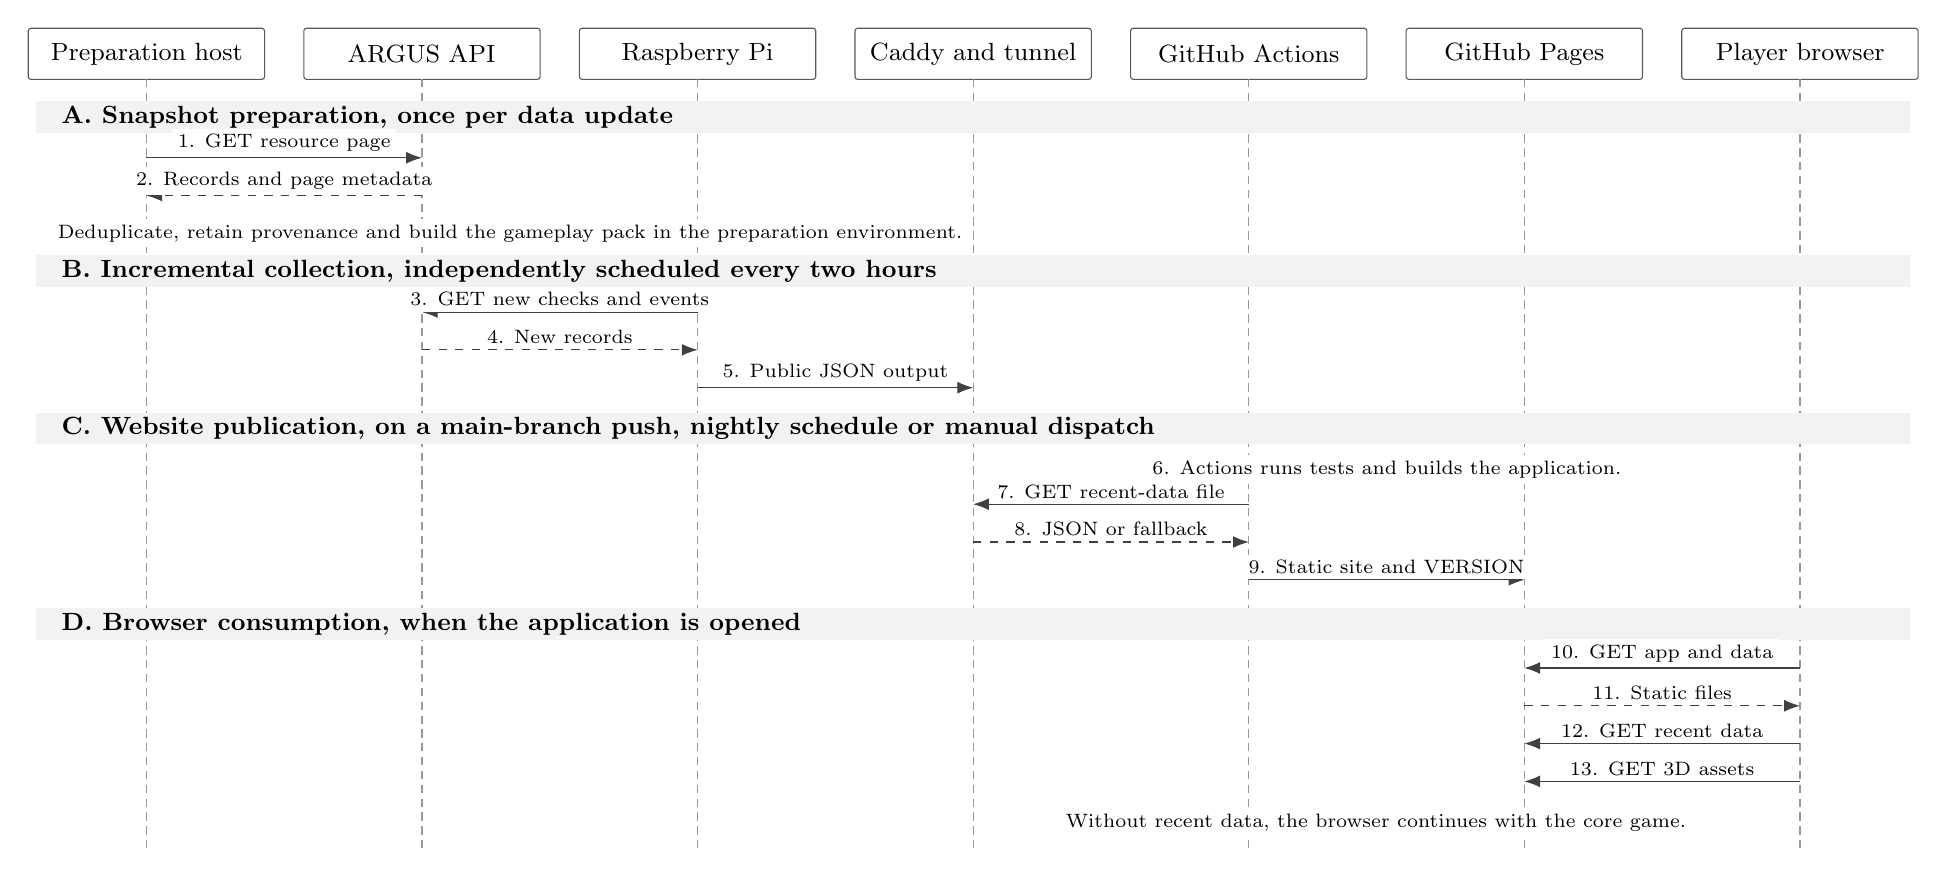
\begin{tikzpicture}[x=1cm,y=0.8cm]
\foreach \x/\name in {0/Preparation host,3.5/ARGUS API,7/Raspberry Pi,10.5/Caddy and tunnel,14/GitHub Actions,17.5/GitHub Pages,21/Player browser}{
 \node[box,text width=2.65cm,font=\small,minimum height=.65cm] at (\x,0) {\name};
 \draw[densely dashed,black!40] (\x,-.4) -- (\x,-12.7);
}
\fill[black!5] (-1.4,-.75) rectangle (22.4,-1.25);
\node[anchor=west,font=\small\bfseries] at (-1.2,-1) {A. Snapshot preparation, once per data update};
\draw[flow] (0,-1.65) -- node[tag,above]{1. GET resource page} (3.5,-1.65);
\draw[flow,dashed] (3.5,-2.25) -- node[tag,above]{2. Records and page metadata} (0,-2.25);
\node[tag,anchor=west] at (-1.2,-2.85) {Deduplicate, retain provenance and build the gameplay pack in the preparation environment.};
\fill[black!5] (-1.4,-3.2) rectangle (22.4,-3.7);
\node[anchor=west,font=\small\bfseries] at (-1.2,-3.45) {B. Incremental collection, independently scheduled every two hours};
\draw[flow] (7,-4.1) -- node[tag,above]{3. GET new checks and events} (3.5,-4.1);
\draw[flow,dashed] (3.5,-4.7) -- node[tag,above]{4. New records} (7,-4.7);
\draw[flow] (7,-5.3) -- node[tag,above]{5. Public JSON output} (10.5,-5.3);
\fill[black!5] (-1.4,-5.7) rectangle (22.4,-6.2);
\node[anchor=west,font=\small\bfseries] at (-1.2,-5.95) {C. Website publication, on a main-branch push, nightly schedule or manual dispatch};
\node[tag,anchor=west] at (12.7,-6.6) {6. Actions runs tests and builds the application.};
\draw[flow] (14,-7.15) -- node[tag,above]{7. GET recent-data file} (10.5,-7.15);
\draw[flow,dashed] (10.5,-7.75) -- node[tag,above]{8. JSON or fallback} (14,-7.75);
\draw[flow] (14,-8.35) -- node[tag,above]{9. Static site and VERSION} (17.5,-8.35);
\fill[black!5] (-1.4,-8.8) rectangle (22.4,-9.3);
\node[anchor=west,font=\small\bfseries] at (-1.2,-9.05) {D. Browser consumption, when the application is opened};
\draw[flow] (21,-9.75) -- node[tag,above]{10. GET app and data} (17.5,-9.75);
\draw[flow,dashed] (17.5,-10.35) -- node[tag,above]{11. Static files} (21,-10.35);
\draw[flow] (21,-10.95) -- node[tag,above]{12. GET recent data} (17.5,-10.95);
\draw[flow] (21,-11.55) -- node[tag,above]{13. GET 3D assets} (17.5,-11.55);
\node[tag,anchor=west] at (11.6,-12.2) {Without recent data, the browser continues with the core game.};
\end{tikzpicture}

\caption{Representative sequence of snapshot acquisition, incremental collection, static publication and browser consumption. Horizontal bands separate independently scheduled processes; they do not imply that a snapshot is refreshed at every live-reader invocation. Return arrows show representative responses, and the text specifies retries, validation and fallback behaviour.}
\label{fig:sequence}
\end{figure}
\vfill
\begin{center}\small\thepage\end{center}
\end{landscape}
\end{document}
